\documentclass[12pt]{article}
%#Scott Pratt, Eren Erdogan, Ekaksh Kataria 2023
\usepackage{subfiles}
\usepackage{indentfirst}
\usepackage{graphicx}
%\usepackage[anythingbreaks,hyphenbreaks]{breakurl}
\usepackage{xurl}
%\usepackage{pdfsync}
\usepackage{amssymb}
\usepackage{amsmath}
\usepackage{bm}
\usepackage[utf8]{inputenc}
\numberwithin{equation}{section} 
\numberwithin{figure}{section} 
\usepackage[small,bf]{caption}
%\usepackage{fontspec}
%\usepackage{textcomp}
%\usepackage{color}
\usepackage{fancyhdr}
\setlength{\headheight}{16pt}
\usepackage[toc,page]{appendix}
%\usepackage[headheight=110pt]{geometry}
\usepackage{bm}

\usepackage[most]{tcolorbox}
\tcbset{
frame code={}
center title,
left=0pt,
right=0pt,
top=0pt,
bottom=0pt,
colback=gray!25,
colframe=white,
width=\dimexpr\textwidth\relax,
enlarge left by=0mm,
boxsep=5pt,
arc=0pt,outer arc=0pt,
}
\newcounter{examplecounter}
\counterwithin{examplecounter}{section}
\setcounter{examplecounter}{0}
\newcommand{\example}[2]{\begin{tcolorbox}[breakable,enhanced]
\refstepcounter{examplecounter}{
\bf Example \arabic{section}.\arabic{examplecounter}:}~~{\bf #1}\\
{#2}
\end{tcolorbox}
}

%\newcommand{\exampleend}{
%\begin{samepage}
%\nopagebreak\noindent\rule{\textwidth}{1pt}
%\end{samepage}
%}

%\usepackage{silence}
%\WarningFilter{hyperref}{Token not allowed in a PDF String}

\newcommand\eqnumber{\addtocounter{equation}{1}\tag{\theequation}}

\newcommand{\solution}[1]{ }

\usepackage{comment}
\parskip 4pt
\parindent 10pt
\textwidth 7.0in
\hoffset -0.8in
\textheight 9.2in
\voffset -1in

%\newcommand{\bm}{\boldmath}
\boldmath

%
\begin{document}


\begin{titlepage}
   \begin{center}
       \vspace*{1cm}

       \textbf{User Manual}

       \vspace{2.0cm}

       \textbf{Scott Pratt, Eren Erdogan, Ekaksh Kataria}
       
       \vfill
            
       \vspace{0.8cm}
     
       
\includegraphics[width=0.4\textwidth]{FRIB_logo.png}
            
            
   \end{center}
\end{titlepage}
\tableofcontents

\newpage


\section{Overview}


 % Motivation behind this program and its uses

This manual describes how to install and run the Smooth Emulator software. The software performs three basic functions. First, the Simplex sampler simply chooses a set of points in model parameter space, at which full model runs will be performed to then tune the emulator. The user must provide a description of the model parameters and the prior in a text files in a standard format. There are several options, the first of which is to choose the points that represent a simplex, e.g. an equilateral triangle in two dimensions or a tetrahedron in three dimensions. In a simplex, all points are equi-distant from one another.  The number of training points is then determined as well. In addition to the standard simplex, there are additional options which are motivated by the simplex form. For the simplex form, if there are $N_p$ model parameters, there are $N_p+1$ training points in the simplex, which matches the number of points needed to determine a linear fit. Another choice, which is based on the simplex chooses enough points to determine a quadratic fit, $(N_p+1)(N_p+2)/2$. The software will write the information about the training points in a standard format, which is described in the manual.

 If the user decides to use training points from a different procedure, the user can still write the information about the points in a different format, and the emulator tuning will still work, as the emulator itself is not predicated on a specific choice of training points. The user is then responsible for running the full model at the training points and expressing observables for each training points in a standard format. The manual describes the output format.

 The second functionality of the software is to build and tune the emulator. Once the observables are calculated at the training points, the emulator will be built and tuned. User input mainly consists of altering a text file of parameters, which provide the user several choices in how the emulator functions. After being trained, the Taylor coefficients representing the emulator are written to a file. One can always add additional training points, and retrain the emulator. 

The third functionality of the software is to perform a MCMC exploration of parameter space using the emulator. This user must express the experimental observables and their uncertainties in a standard format. The MCMC software will read the emulator coefficients from file and perform the MCMC exploration. This procedure is also guided by a simple text file of parameters. The MCMC software uses python and Matplotlib to generate plots that describe the posterior. 

\section{Getting Started}\label{sec:simplex}

\subsection{Installation}

Smooth Emulator software should run on UNIX, Mac OS or Linux, but is not supported for Windows OS.

\begin{description}
\item[Step 0 : Prerequisites] 
\end{description}

Smooth Emulator is largely a C++ project. In addition to a C++ compiler, the user needs the following software installed.

\begin{itemize}
    \item git
    \item CMake
    \item Eigen3 (Linear Algebra Package)
    \item GSL (Gnu Scientific Library)
    \item Python/Matplotlib (only for generating plots in the MCMC procedure)
\end{itemize}

CMake is an open-source, cross-platform build system that helps automate the process of building, testing, and packaging software projects. It provides a simple and efficient way to generate platform-specific build files from a platform-independent configuration. Hopefully, CMake will perform the needed gymnastics to find the Eigen3 and GSL installations. To install CMake, either visit the CMake website (https://cmake.org/), or use the package manager.

Eigen is a C++ template library for vector and matrix math, i.e. linear algebra. The user can visit the Eigen website (https://eigen.tuxfamily.org/dox/), or use their system's package manager.

The GNU Scientific Library (GSL) is a numerical library for C and C++ programmers. The library provides a wide range of mathematical routines such as random number generators, special functions and least-squares fitting. There are over 1000 functions in total with an extensive test suite. One can either download the software from the GSL website (https://www.gnu.org/software/gsl/), or use a package manager.



\begin{description}
\item[Step 1 : Making Home Directory and Setting Home Environment Variable]
\end{description}

The software requires two repositories. They should be cloned into the same directory. For compilation purposes this directory needs to be accessed via an environmental directory.  For example the directory might be named {\tt githome\_msu} (another name would be fine, just substitute it everywhere below). First, create the directory, then enter that directory.
{\tt 
\begin{verbatim}
    % mkdir (some path)/githome_msu
    % cd (some path)/githome_msu
\end{verbatim}
}
Then, create an environmental variable which describes the location of the directory above. 

{\tt 
\begin{verbatim}
    % export GITHOME_MSU=(some path)/githome_msu
\end{verbatim}
}
It is recommended to copy this command into the user's .bashrc (or equivalent) file to avoid re-enerting it each time one needs to recompile.

\begin{description}
\item[Step 2 : Downloading and Compiling] 
\end{description}
{\tt 
\begin{verbatim}
    % git clone https://github.com/scottedwardpratt/smooth.git
    % git clone https://github.com/scottedwardpratt/commonutils.git
\end{verbatim}
}

This creates 2 directories: {\tt .../msu\_git/commonutils} and {\tt .../msu\_git/smooth}. Next, create the Make files with cmake, then compile them.
{\tt 
\begin{verbatim}
    % cd ../githome_msu/commonutils/software
    % cmake .
    % cd ../githome_msu/smooth/software
    % cmake .
    % cd ../githome_msu/smooth/program
    % cmake .
    % make simplex
    % make smoothy_writecoefficients
    % make smoothy_readcoefficients
\end{verbatim}
}
As described further below, the foundational software and libraries are in the {\tt githome\_msu/ commonutils/software} and {\tt githome\_msu/smooth/software} directories. The {\tt githome\_msu/smooth /program} directory has the short programs which call functions from the other directories. This arrangement should more easily allow the reader to copy the codes in {\tt programs} directory to make their own versions.

\begin{description}
\item[Step 3 : Making a Project Directory] 
\end{description}
{\tt 
\begin{verbatim}
    % cp -r ../template myproject
\end{verbatim}
}
     
This will set up the directory structure for use.  \\ 

\begin{description}
\item[Step 4 : CMake]
\end{description}

{\tt 
\begin{verbatim}
    cmake /path/to/project
\end{verbatim}
}

\subsection{Structure}

The directory structure of the repository is as follows: 

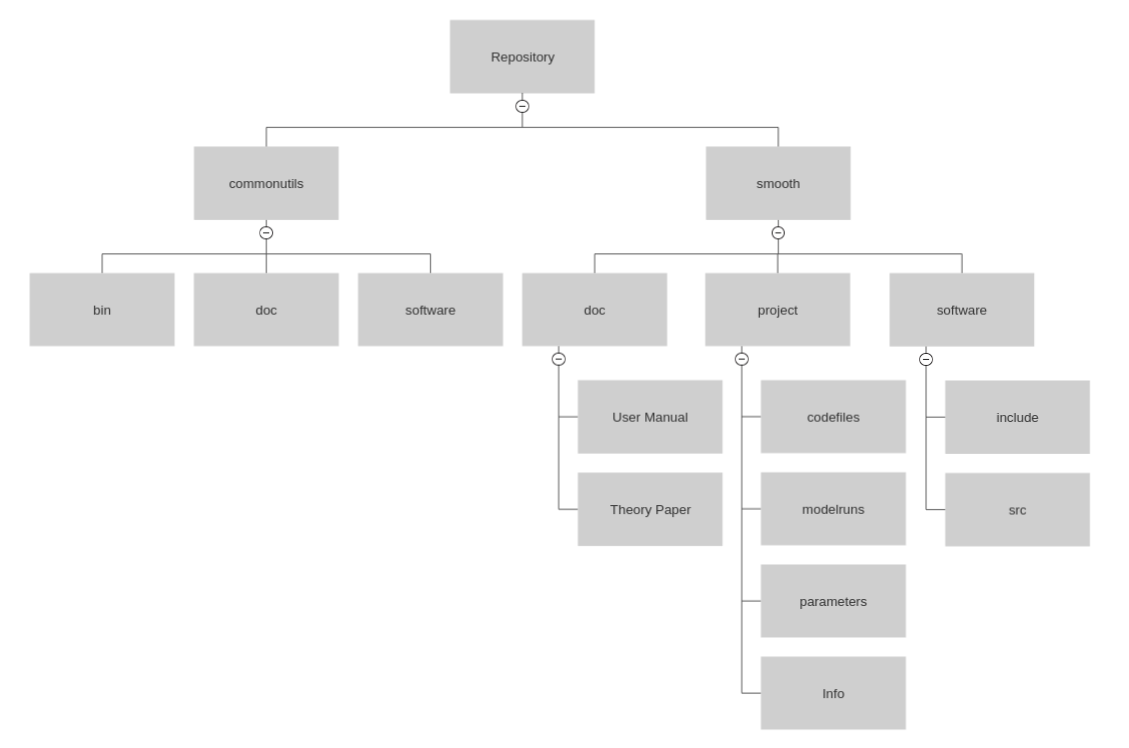
\includegraphics[width = 120mm]{Structure_Tree.png}

\subsubsection{Software Directory}

The software file contains all the classes and the main functionality of the emulator. The Software file contains the two main directories, the Include directory and the source directory called src.

\subsubsection{Include Directory}

This directory contains all the header files. The header files contain a set of predefined library functions and newly defined classes for the different functions used in the emulator code. 

\subsubsection{Source Directory (Src)}

Within this directory, you will find the core functions of the emulator in the form of .cc files. Each step of the process has its own class with distinct constructors. These .cc files reference the corresponding .h file using the "\#include" feature and then define each class with unique initial values, methods, and constructors. 


\subsubsection{Project Directory}

The project directory is where the emulator works. There are files in this directory: 

1. Info Directory 

The Directory includes the parameter and observable file with SigmaA values for referencing the expected values of added parameters and observables by the user. These values represent the standard deviation of the Gaussian distribution that is used to sample the emulator coefficients A during the tuning process.

The value of SigmaA controls the step size of the random walk in the parameter space during the MCMC sampling. A larger SigmaA means larger jumps in the parameter space, leading to faster exploration of the space but possibly sacrificing the accuracy of the tuning process. Conversely, a smaller SigmaA leads to smaller steps, which may improve accuracy but may also slow down convergence.

\begin{description}
\item[Template Project Directory] \

\ 1. simplex.cc \\
\ This cc helps in choosing the training points and making the model parameters and creates the model run directory using the prior info for the simplex 

\ 2. fakemodel.cc \\
\ The fakemodel.cc is a template used to represent a potential model. It will be replaced by the actual model created by the user. 

\ 3. smoothy.cc 
\ This cc files read in the parameter files and reads in the training point info from the simplex and tune the function Y values and generate the coefficient for each observable and make a directory of the possible coefficient values 

\ 4. smoothy\_readcoefficients.cc 
\ This cc file reads in the coefficient files and reads in the training info from the simplex and tests the samples from the emulator at the training points. 

\end{description}

The order in how the code works is mentioned in the next section 


\subsection{Usage}
\label{sec:Usage}

The user is required to have some knowledge of C++ in order to write a routine program that calls methods from the software directory for their needs. Some example codes can be viewed in the template directory.

\section{Simplex}

\subsection{Summary}
From the motivation, we can interpret that the purpose of the simplex is to produce training points. The emulator will use these training points to tune itself, and output results. Thus, it is important that one takes their time, and chooses how they want to generate their training points carefully.

The user first needs to make sure that they follow the instructions under Section \ref{sec:Usage}. After this, one should decide on how they want to generate their training points. The code provides the user with different options, but one can choose to generate the training points in a different way as well.

For training point generation we use the file simplextest.cc. The functionality, how to use and the output of these files are explained below.

\subsection{Training Point Generation}

Simplex is a mathematical term that generalizes the notion of a triangle or a tetrahedron to arbitrary dimensions. The simplex method uses the vertices of simplexes to get training points at different radii along the edges. This method also is computationally cheap due to its iterative process.

To use the simplex method, use the following command in the terminal window:

{\tt
{
\begin{verbatim}
    simplextest parameters/emulator_parameters.txt
\end{verbatim}
}}

This code is also responsible for generating the directory that the run files are stored. The stored values will be the values that used in the emulator.

\section{Tuning the Emulator}

\subsection{Summary}

From the motivation, we can interpret that the purpose of the emulator is to reproduce the model reasonably away from the training points and the goal is to focus on a particular class of functions that are smooth. 

The emulator has a specific functional form with numerous coefficients denoted as $A_{\vec{n}}$. The theory of steps illustrated on how to constrain the emulator is mentioned in the theory section below.  After Running the simplex.cc file we output the model\_par.txt files for each run using the prior information using the number of parameters sent from the model\_parameter.txt file from the info directory and use the simplex to create the training points.

\subsection{Code}

For training the emulator we create the coefficient samples using the smoothy
\_writecoefficients.cc. The Functionality, how to use and the output of these files are explained below.

The fakemodel.cc is a template used to represent a potential model. It will be replaced by the actual model created by the user. The file reads in the model prior info and the observable info files from the info directory and generates the observable text files in the run directory. 
 
\subsection{Writing Coefficients}

In the terminal window run the following command after the simplex and importing the model.

{\tt 
\begin{verbatim}
smoothy parameters/emulator_parameters.txt 
\end{verbatim}
}

This code is responsible for invoking the primary functionality that adjusts the training points for the model. It generates coefficient samples, which are then organized in a coefficient directory within the project directory. The directory contains information about each observable and samples of various coefficient values. The following methods are used to accomplish this task:

This code reads in the values from each run directory and stores the values of the observables and the parameters values and stores in the current code. 

The purpose of this function is to perform a Markov Chain Monte Carlo (MCMC) parameter tuning process to optimize some coefficients of a smooth emulator. The code attempts to find the best set of coefficients that maximize the log probability of the emulator given some training data. 

Final Output and Results:
After completing the specified number of iterations, the algorithm calculates the success percentage (proportion of successful updates), the final value of SigmaA, and the log-likelihood normalized by the number of degrees of freedom (Ndof) for the best parameter set (BestLogP/Ndof). These results are displayed in the console using CLog::Info(). 

Interpreting the Results:
The success percentage gives an indication of the acceptance rate of new parameter sets during the MCMC process. A higher success rate generally indicates efficient parameter tuning. The value of SigmaA represents the estimated uncertainty or spread in the parameter space. The BestLogP/Ndof provides a measure of the goodness of fit achieved by the best parameter set. 


The function also updates statistics for the sampled variance (SigmaA) to calculate the average variance (SigmaAbar) over all the generated samples. In summary, GenerateASamples iteratively tunes the coefficients using MCMC and stores the optimized coefficient samples in a matrix for further analysis. It is used for the process of generating and analyzing samples for the smooth emulator.

The Code also Logs the comparison between the predicted value and the actual training data value for the current observable. Also, log the corresponding uncertainty. The function evaluates the smooth emulator's accuracy by generating predictions for each observable at the training points and comparing these predictions with the actual training data.  


The code also writes metadata about the number of parameters (NPars), maximum rank (MaxRank), and total number of coefficients (NCoefficients) to a file named "meta.txt" in the created directory. For each sample generated using the GenerateASamples() function, the function writes the corresponding coefficients (parameters) to a separate file named "sampleX.txt" in the created directory, where "X" represents the sample index. The number of coefficients is equal to smooth $\rightarrow$ NCoefficients, and they are written in a column-wise format. 


\section{MCMC}


\section{Troubleshooting}


\section{Theory}

\begin{description}
\item[Constraining the emulator] \
\\
\ 1. $M$ full model runs are conducted at different positions $\vec{\theta}_{m=1,M}$. These runs provide corresponding values $F_{m=1,M}$. 

\ 2. The functional form of the emulator has a large number of coefficients $A_{\vec{n}}$, which exceeds the number of training points M. However, the dependence of the coefficient A is purely linear. 

\ 3. The coefficients are enumerated as $A_c$ with $c=1\cdots C$, where $C>M$.

\ 4. Random values are assigned to the coefficients $A_M$ through $A_C$, excluding the first $M$ coefficients. 

\ 5. A set of linear equations is solved to determine the values of the first $M$ coefficients. This process involves finding the coefficients that best fit the training points. 

\ 6. A weight is applied to the values of $A$, taking into account their consistency with the prior likelihood of $A$ and the given constraints. This step helps to incorporate prior knowledge and constraints into the emulator. 

\ 7. A representative set of A is generated, typically consisting of a dozen samples. Each sample function passes through all the training points but may deviate further from them. 

\ 8. By averaging over $N_{\rm sample}$ sets of coefficients, a prediction for the emulator can be made at a specific point $\theta$. The $N_{\rm sample}$ points provide an estimate, and their variance represents the uncertainty associated with the emulator's prediction. 

\end{description}\




\appendix


\section{Parameter Map}
The parameter map is the file user changes in order to use and optimize the code according to the model the user has and the output user is expecting. The parameters described below can be found in the parameter directory and in the file emulator\_parameter.txt.

The parameter map has a prefix for each of the parameters SmoothEmulator and in the appendix they are mentioned direcotry 

\subsection{NTrainingPts}
 The number of training points determines how many data points are available for training the smooth emulator. It affects the number of training samples used in various calculations and tuning steps, and ultimately influences the accuracy and generalization ability of the emulator model. 

A larger number will lead to a more accurate emulator, but it could also increase computational costs. The choice of the number depends on the specific application and the trade-off between accuracy and efficiency.


\subsection{SigmaYMin}
 
This value is used to set a lower limit for SigmaY, it might be used to prevent the emulator from overfitting or producing unrealistic predictions by penalizing or restricting very small uncertainties in the observed data. 



\subsection{NMC}

This parameter specifies the number of iterations (steps) to be performed in the MCMC algorithm which is used for tuning the emulator parameters to find the optimal values that maximize the likelihood of the observed data. A larger value of NMC allows for a more thorough exploration of the parameter space, potentially leading to more accurate tuning results.

However, it also increases the computational cost of the tuning process since each iteration requires calculating the emulator output and evaluating the likelihood.

The choice of NMC should be made carefully to strike a balance between the accuracy of the tuning results and the computational efficiency of the algorithm. The optimal value of NMC may depend on the complexity of the problem, the size of the training data, and the available computational resources.  




\subsection{NASample}

This parameter represents the number of samples generated from the smooth emulator to estimate uncertainty in the emulator predictions. It controls the number of times the emulator coefficients (A) are sampled to obtain multiple emulator outputs.

The value of the NASample should be chosen based on the desired level of confidence in the emulator predictions and the computational resources available. Larger values of the NASample generally provide more reliable uncertainty estimates but also require more computational time to generate the samples.  


\subsection{MCStepSizeis}
 This parameter controls the step size of the Metropolis-Hastings Markov Chain Monte Carlo (MCMC) algorithm during the tuning process.
 
A larger value of MCStepSize means larger steps, which can lead to faster exploration of the parameter space but might also result in less precise tuning. Smaller MCStepSize leads to smaller steps, which may improve accuracy but may require more iterations to fully explore the parameter space.

\subsection{MCSigmaAStepSize}
 This parameter controls the step size for updating the standard deviation SigmaA during the Metropolis-Hastings Markov Chain Monte Carlo (MCMC) algorithm's tuning process. 

This enables the algorithm to simultaneously find the optimal values of A and SigmaA that best fit the training data and provide accurate emulator predictions.


 
\subsection{TuneChooseMCMC}

This boolean parameter that controls the choice of tuning method used in the smooth emulator. The choice between MCMC and "perfect" tuning methods can significantly impact the accuracy and computational efficiency of the emulator.

The MCMC method is more robust and can handle complex parameter spaces, but it requires a larger number of iterations (NMC) and can be computationally expensive. On the other hand, the "perfect" tuning method may be faster, but it may not fully explore the parameter space and may not find the global optimum. \\



\subsection{UseSigmaYRreal}  

This is also a boolean parameter that determines whether the true (real) standard deviation (SigmaY) of the observed data is used during the parameter tuning process of the smooth emulator.

By considering the true standard deviation SigmaY in the likelihood calculation, the tuning process accounts for the uncertainty in the observed data. This can lead to more accurate parameter tuning and better emulator predictions, especially when the true standard deviation is known and informative about the variability in the observed data.



\subsection{ConstrainA0}
 This boolean parameter controls whether the emulator coefficients $A_i$ are constrained during the tuning process. Specifically, it determines whether the first coefficient $A_0$ is fixed or allowed to vary during the tuning iterations.  

For some problems, it may be known or desired that the first coefficient $A_0$ should take a specific value based on physical constraints or prior knowledge. In such cases, setting the parameter to true ensures that the tuning process respects this constraint.

On the other hand, if there is no specific reason to constrain $A_0$, setting the parameter to false allows the tuning algorithm to explore the full parameter space, including the possibility of $A_0$ taking different values, which might lead to better-fitted emulator coefficients.\\

\subsection{CutoffA}
This parameter sets the extra width that keeps sigma A from drifting off to infinity.  

\subsection{LAMBDA}

This parameter represents a regularization term used in the smooth emulator for tuning the model coefficients (A). The term "LAMBDA" is typically used to denote the smoothness parameter and it serves as a tuning knob to control the complexity of the smooth emulator model.

The Lamda helps control the trade-off between fitting the training data accurately and keeping the model complexity in check. A higher value of LAMBDA leads to a more regularized (smoother) model with simpler coefficients, while a lower value allows the model to adapt more to the training data, potentially leading to more complex and flexible coefficients. It is often determined through experimentation and fine-tuning to achieve the best balance between model accuracy and complexity.

\subsection{ModelRunDirName}
It is a string variable that stores the name of the directory where the smooth emulator stores the information related to a specific model run.    \\

\subsection{CoefficientsDirName} 
It is a string variable that stores the name of the directory where the smooth emulator stores the coefficients (parameters) obtained during the tuning process.   \\

\subsection{MAXRANK}

It is a variable that represents the maximum rank allowed for the smooth emulator and it determines the number of basis functions used to represent the smooth functions during the modeling process. 

A higher MAXRANK allows the emulator to capture more complex and flexible response surfaces, but it may require more data points and computational resources. Conversely, lower MAXRANK results in a simpler model with reduced flexibility but may be more computationally efficient and require fewer data points.


\subsection{UseRFactor}
It is a boolean parameter that determines whether the smooth emulator uses an "R-factor" regularization term during the tuning process. It is a measure of how well the smooth emulator reproduces the training data points.

By incorporating the R-factor into the tuning process, the emulator can optimize the coefficients (A) in a way that balances the fit to the training data with the overall smoothness of the model.

\subsection{TrainType}
  Determines the training type that the simplex will use. The default type is 1. All types have different uses, pros, and cons. The differences between type are explained below:

  

\subsection{RTrain}



\end{document}
